% Chapter 4 evidence table-image snippets.
% Required packages in the dissertation preamble:
% \usepackage{graphicx}
% \usepackage{float}
%
% Image path assumption:
% These snippets assume the table images are available under:
% figures/chapter4/

% Place Table 4.1 near the beginning of Chapter 4, immediately after the
% Chapter 4 overview subsection and before the first hypothesis section.
\begin{table}[H]
    \centering
    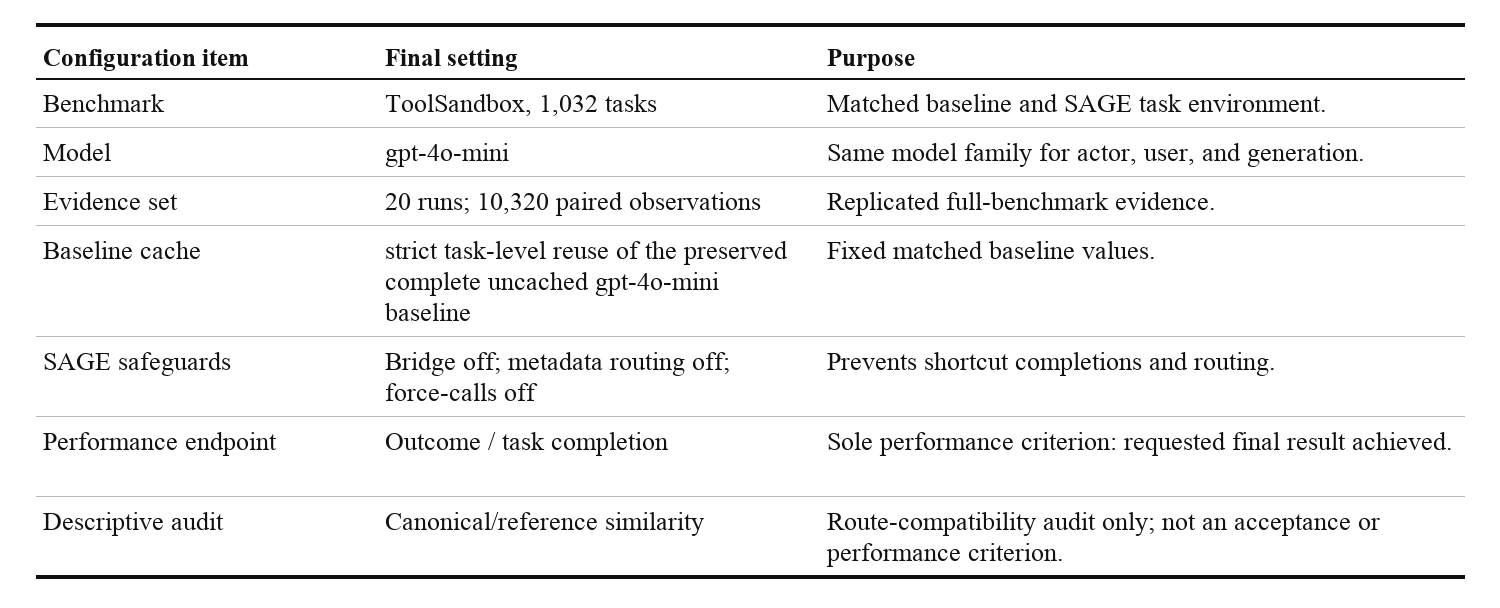
\includegraphics[width=\textwidth]{figures/chapter4/table_4_1_evidence_campaign.png}
    \caption{Archival July campaign settings. The cache description in the rendered table is superseded by the publication correction in Chapter 4.}
    \label{tab:chapter4-evidence-campaign}
\end{table}

% Place Table 4.2 after Table 4.1, before the individual hypothesis
% subsections, to establish the full replication set used in the results.
\begin{table}[H]
    \centering
    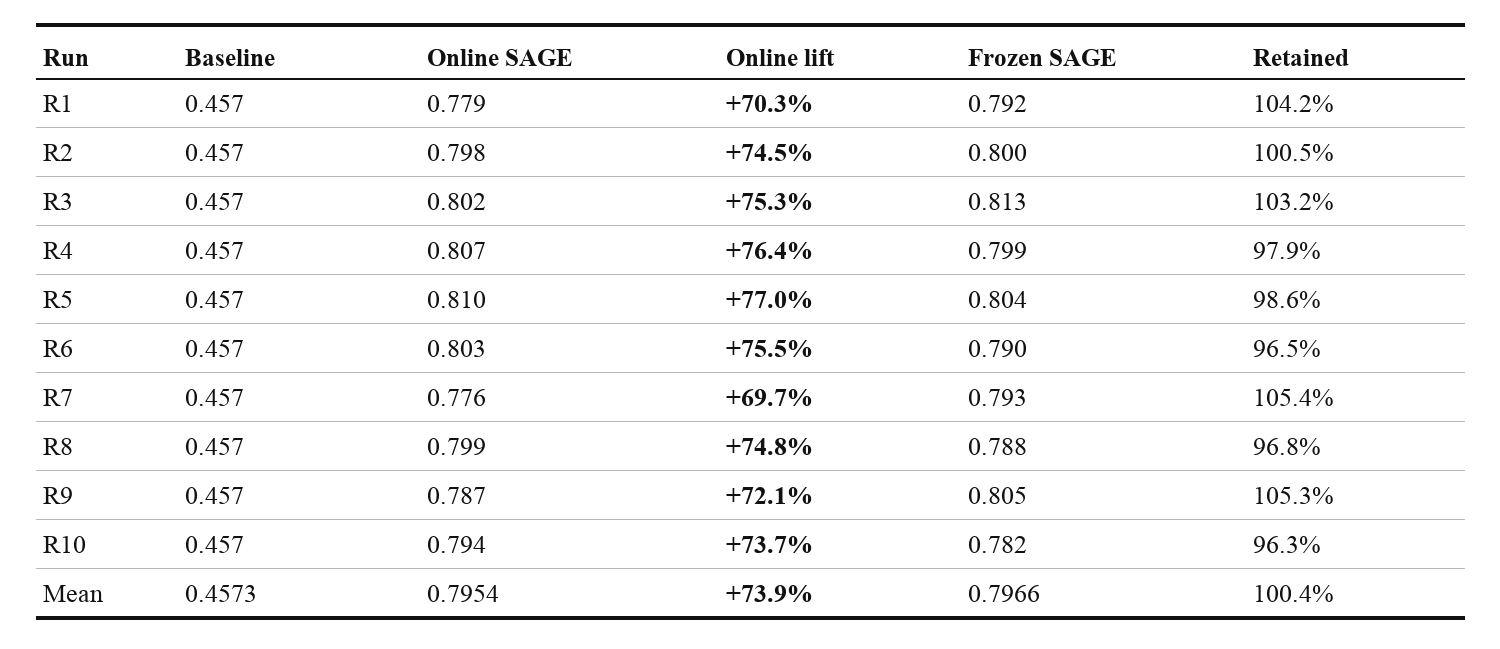
\includegraphics[width=\textwidth]{figures/chapter4/table_4_2_replication_results.png}
    \caption{Historical ToolSandbox replication results; the final row reports means. These values are descriptive pending the strict fresh-control rerun.}
    \label{tab:chapter4-replication-results}
\end{table}

% Place Table 4.3 in the Hypothesis 1 results subsection, after the
% Hypothesis 1 statement and explanation.
\begin{table}[H]
    \centering
    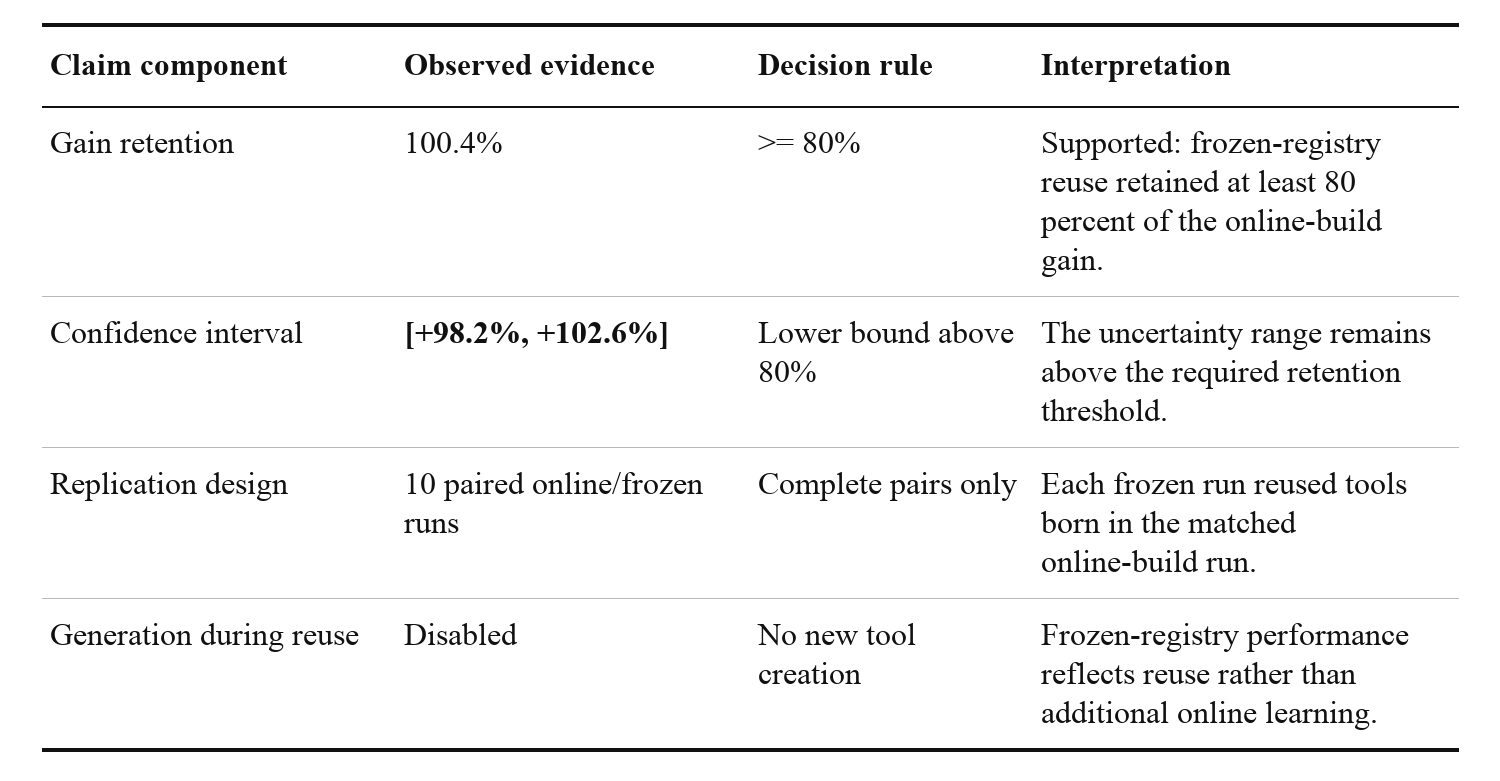
\includegraphics[width=\textwidth]{figures/chapter4/table_4_3_h1_frozen_registry_retention.png}
    \caption{Historical H1 estimate from the superseded hybrid-cache campaign. A hypothesis decision awaits the strict fresh-control rerun.}
    \label{tab:chapter4-h1-frozen-registry-retention}
\end{table}

% Place Table 4.4 in the Hypothesis 2 results subsection, after the
% Hypothesis 2 statement and explanation.
\begin{table}[H]
    \centering
    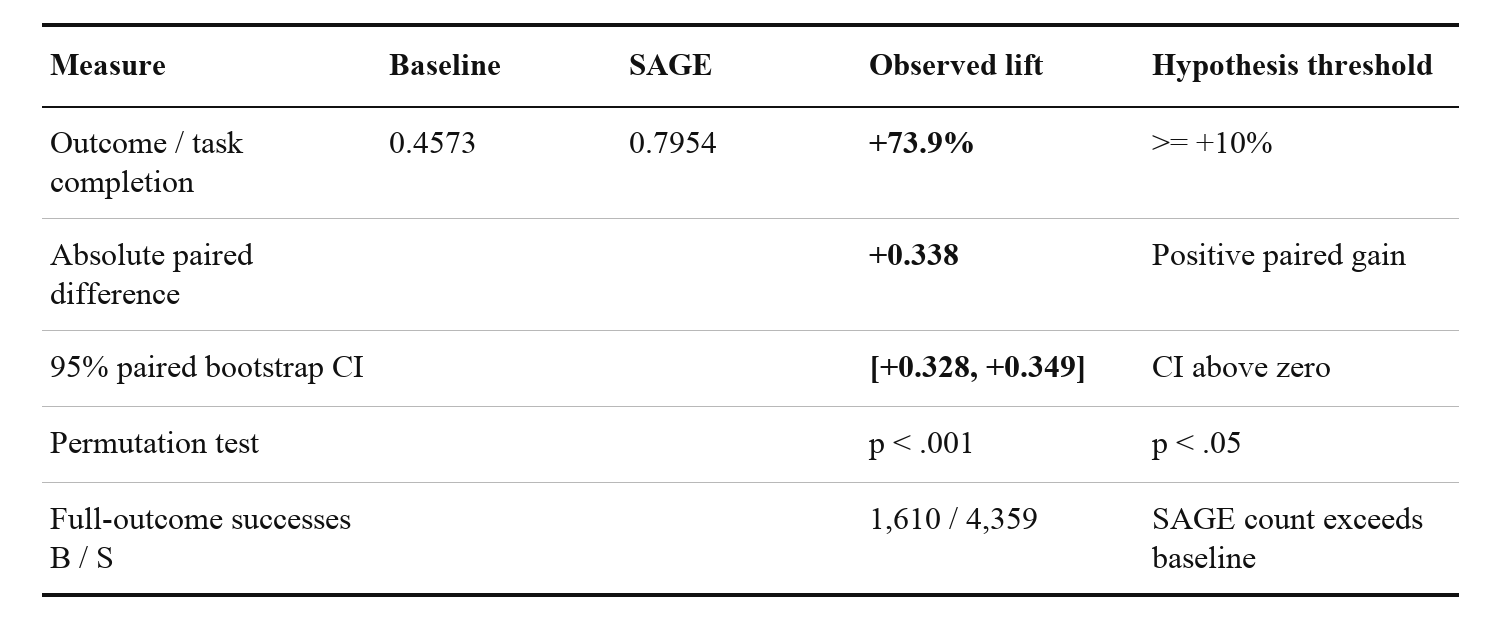
\includegraphics[width=\textwidth]{figures/chapter4/table_4_4_h2_overall_task_completion.png}
    \caption{Historical H2 estimate from the superseded hybrid-cache campaign. A hypothesis decision awaits the strict fresh-control rerun.}
    \label{tab:chapter4-h2-overall-task-completion}
\end{table}

% Place Table 4.5 in the Hypothesis 3 results subsection, after the
% Hypothesis 3 statement and explanation.
\begin{table}[H]
    \centering
    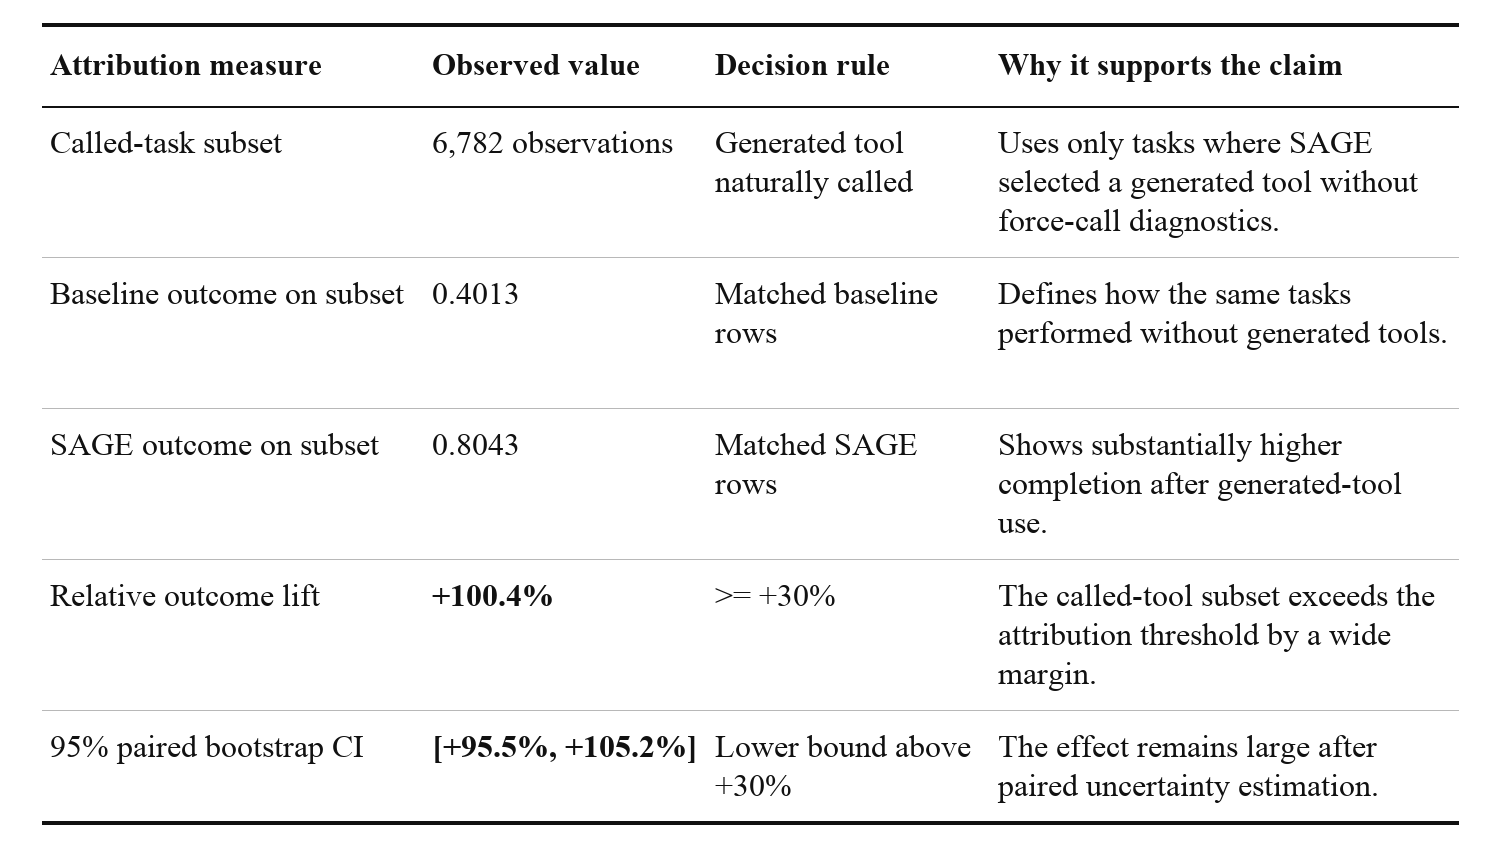
\includegraphics[width=\textwidth]{figures/chapter4/table_4_5_h3_generated_tool_attribution.png}
    \caption{Historical H3 generated-tool-called subset from the superseded hybrid-cache campaign. A hypothesis decision awaits the strict fresh-control rerun.}
    \label{tab:chapter4-h3-generated-tool-attribution}
\end{table}

% Place this table in the Summary of Hypothesis Decisions subsection.
\begin{table}[htbp]
    \centering
    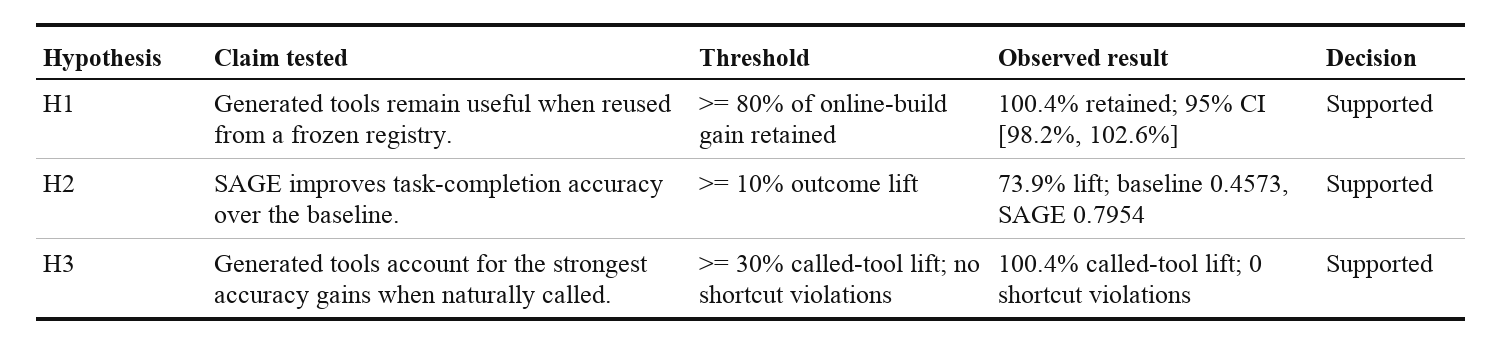
\includegraphics[width=\textwidth]{figures/chapter4/table_4_8_hypothesis_decision_summary.png}
    \caption{Archival July hypothesis decisions, withdrawn pending the strict fresh-control ten-pair rerun.}
    \label{tab:hypothesis-decision-summary}
\end{table}

% Place the generated-tool lifecycle table after the hypothesis decision
% summary, in the Generated Tool Lifecycle Results subsection.
\begin{table}[H]
    \centering
    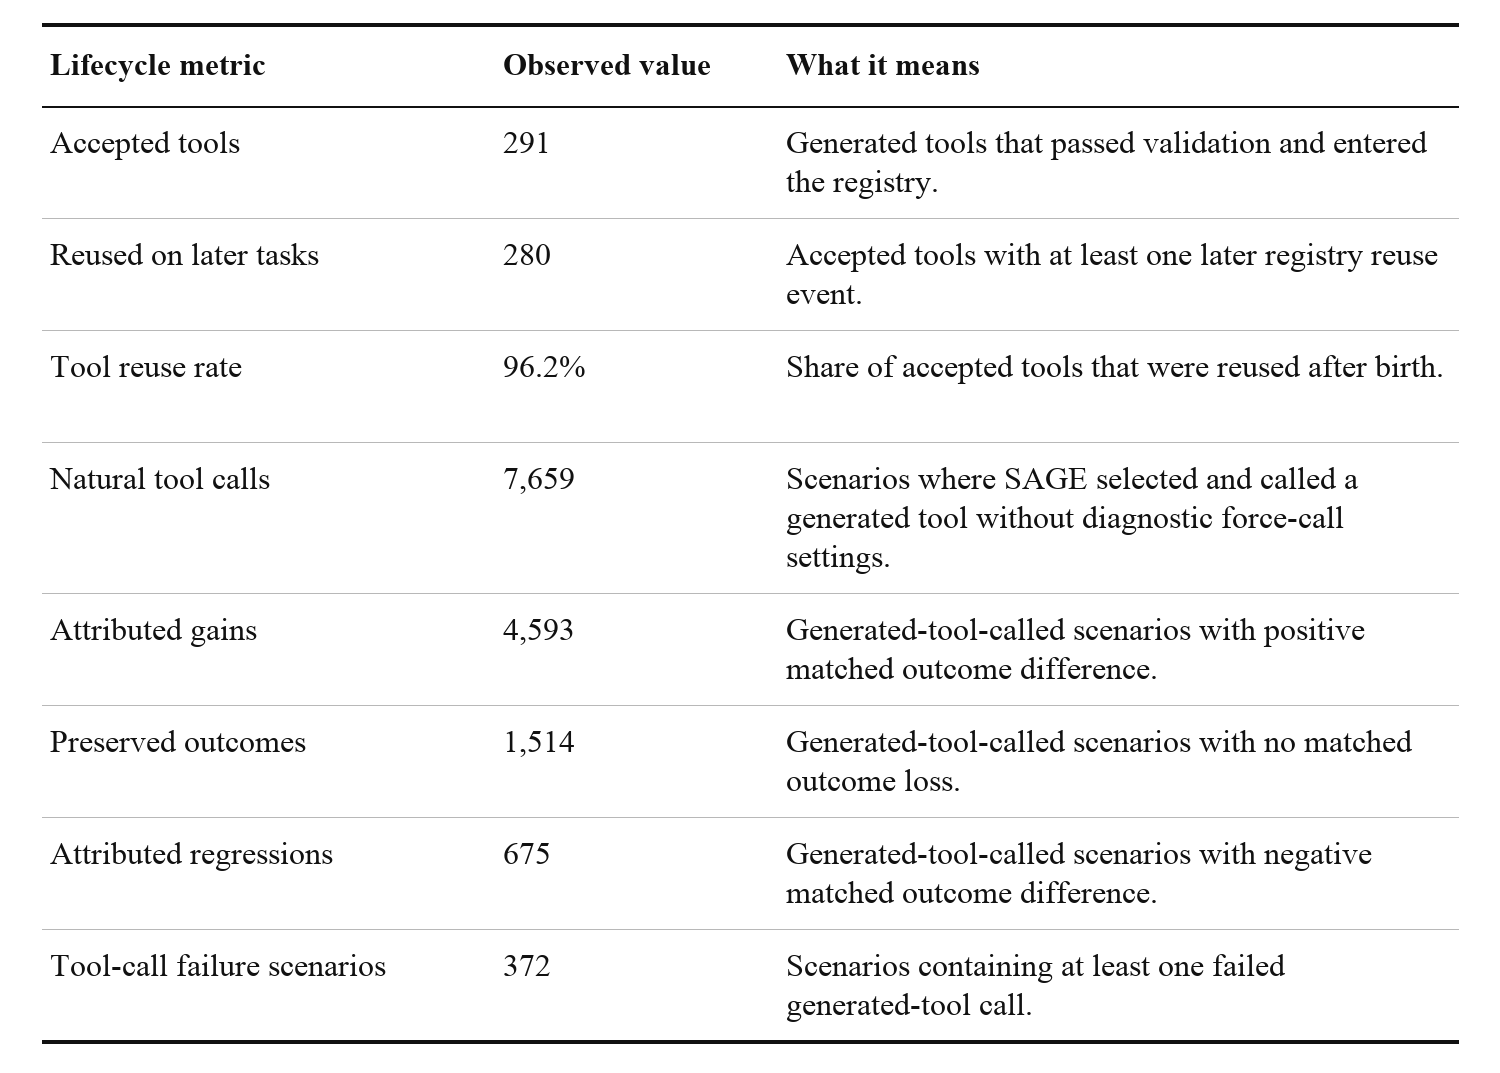
\includegraphics[width=\textwidth]{figures/chapter4/table_4_6_generated_tool_lifecycle.png}
    \caption{Historical generated-tool lifecycle and contribution counts from the superseded campaign; confirmatory interpretation awaits the strict fresh-control rerun.}
    \label{tab:chapter4-generated-tool-lifecycle}
\end{table}

% Place Table 4.7 in the Hypothesis 3 Validity Checks subsection, before
% the Hypothesis 3 interpretation.
\begin{table}[H]
    \centering
    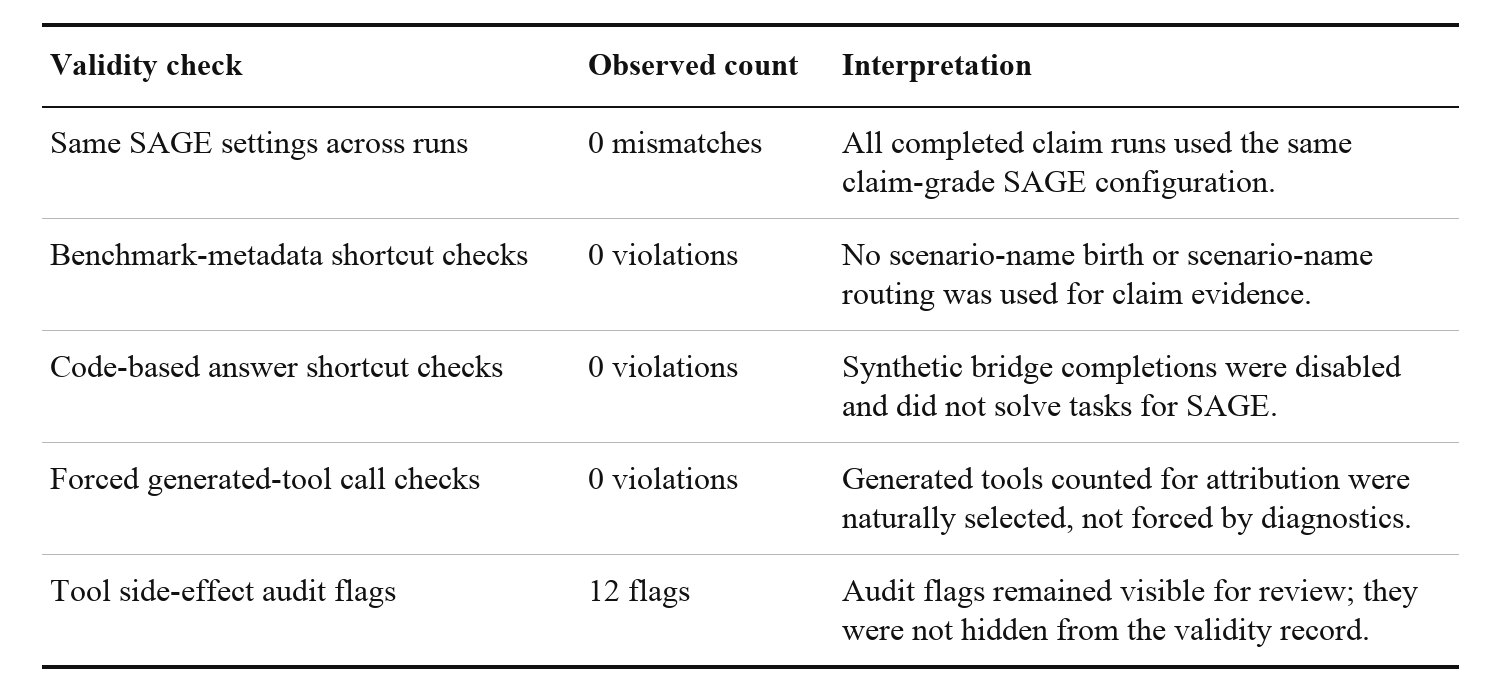
\includegraphics[width=\textwidth]{figures/chapter4/table_4_7_validity_checks.png}
    \caption{Historical validity checks for the superseded July campaign. These safeguards do not remedy the hybrid-control provenance and cache-conditioned reflection defect.}
    \label{tab:chapter4-validity-checks}
\end{table}

% Place Table 4.9 after the generated-tool lifecycle table or in the
% limitations/error-analysis subsection.
\begin{table}[htbp]
    \centering
    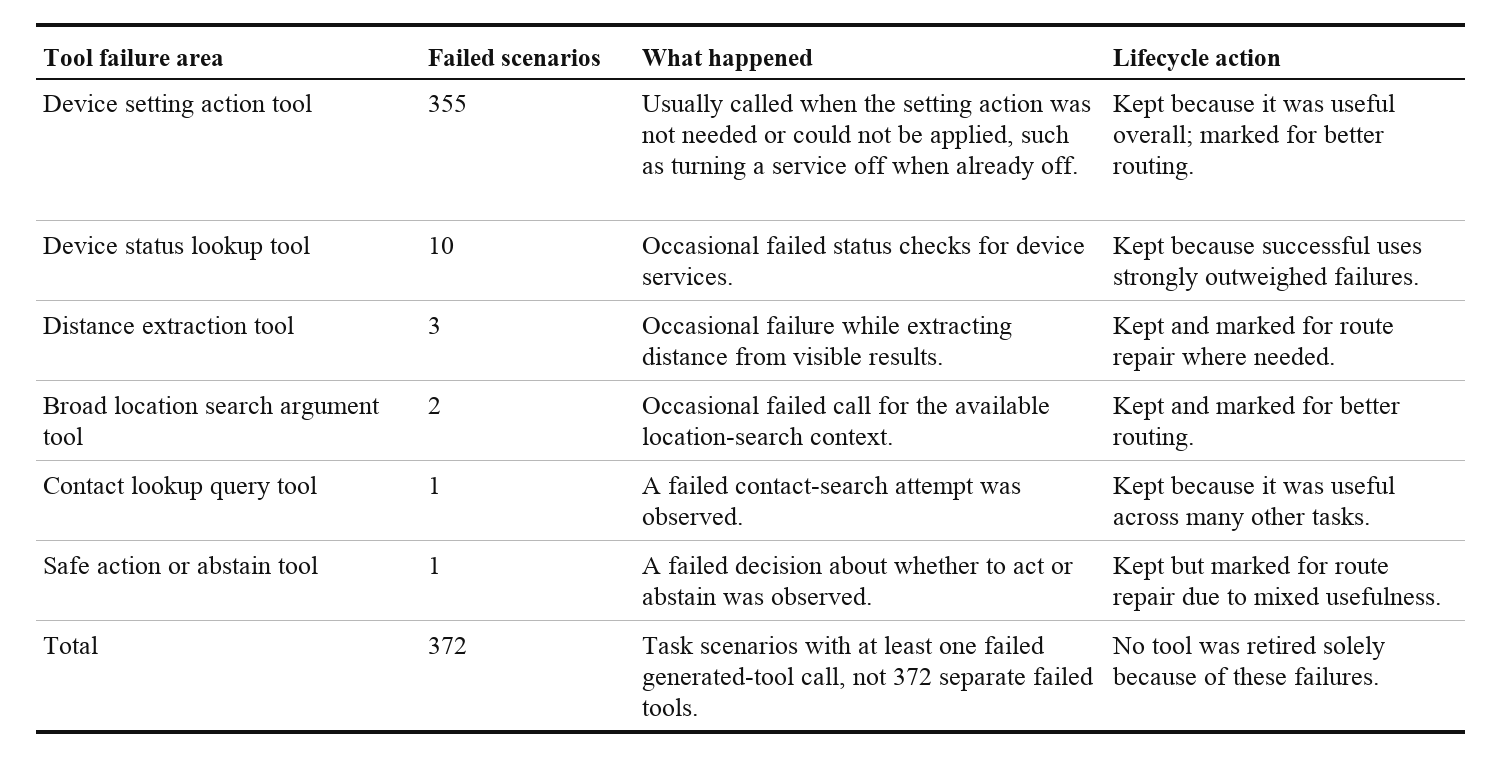
\includegraphics[width=\textwidth]{figures/chapter4/table_4_9_generated_tool_failure_summary.png}
    \caption{Historical generated-tool failure summary across the ten superseded July online-build runs.}
    \label{tab:chapter4-generated-tool-failure-summary}
\end{table}
